\chapter{Technical Background}
\label{chap:technicalbackground}

\section{Introduction}
This section will provide an overview about existing technologies of CI Tech Sensors, namely the ones which are involved and affected by this project.

\section{The NIF File}
NIF stands for \emph{Note Information File} and is a binary file format which stores note transaction records. In other words a NIF file is what you get when processing a set of notes through a banknote reader. The NIF stores Metadata, Note Record Data and Image Data, it thus contains both raw data and data calculated by the reader. It is encoded in a proprietary binary format, which uses a tree-like structure of so called Chunks, parts of data with a unique ID and a fixed length to store and structure data. An example of a  relevant Chunk, which is referenced throughout this documentation is the NOTEMSG2 (Note Message 2, historically because there used to exist a Note Message 1 Chunk) Chunk, which is present once for each note recorded and which contains the most relevant information about a note's recognition and classification by the reader. This information can then be used for labelling our dataset. \par
A NIF has a unique ID (the file's MD5 checksum), which is also called FileID. With the help of the FileID, the NoteID can be defined as the concatenation of the FileID and the note's\footnote{We informally speak of notes but in this context actually do not mean notes as an abstract concept like ``The CHF 10 banknote`` but rather \emph{recordings of physical note}. Simply put: A note is a record of a physical banknote, which was done by a banknote reader and is stored in a NIF file.} FilePosition, which corresponds to the order in which the note's were recorded. Thus
\begin{align*}
8AD47001CC4BD7B49783B4D6125F9551:1
\end{align*}
is the unique ID of the first note (record) in the NIF file with checksum $8AD47001CC4BD7B49783B4D6125F9551$.

\begin{figure}
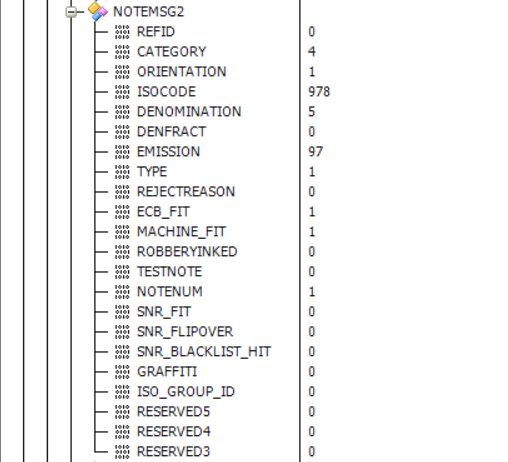
\includegraphics[width=0.35\textwidth]{images/NoteMsg2Chunk}
  \caption{Content of NOTEMSG2 Chunk as displayed in a proprietary ChunkFormat parsing software}\label{fig:notemsg2}
\end{figure}

\section{The CDF file}
The CDF (\emph{Currency Data File}) is a binary parameter file, which contains all the required information to enable the banknote reader to process, classify and validate all banknotes of one currency. It stores metadata as well as algorithmic recognition data, which specifies the algorithms used, their order of execution and the respective parametrization for each algorithm and banknote type. The CDF is released independently of the actual banknote reader software and the development and maintenance of CDFs is one of the main tasks of currency adaptation specialists. Typical reasons why a CDF would need to be adjusted are the release of a new banknote or the emergence of a new type of counterfeit which the CDF needs to be able to detect.

\section{MOVEm File Index}
MFX (MOVEm File Index) is a central index of all files in the Data Pool, allowing the lookup of a file's path in the central Data Lake. MFX is a Flask application with a REST API backend. In addition to allowing the lookup of individual files, it lists the indexed directories as well as duplicate NIF files in the data lake and defect NIF files. Moreover, MFX is integrated into MCM, insofar as MCM has access to the MFX API and can thus load directly from the Data Lake. The following figure visualizes how MFX is used for path lookup within MCM:
\begin{figure}[ht!]
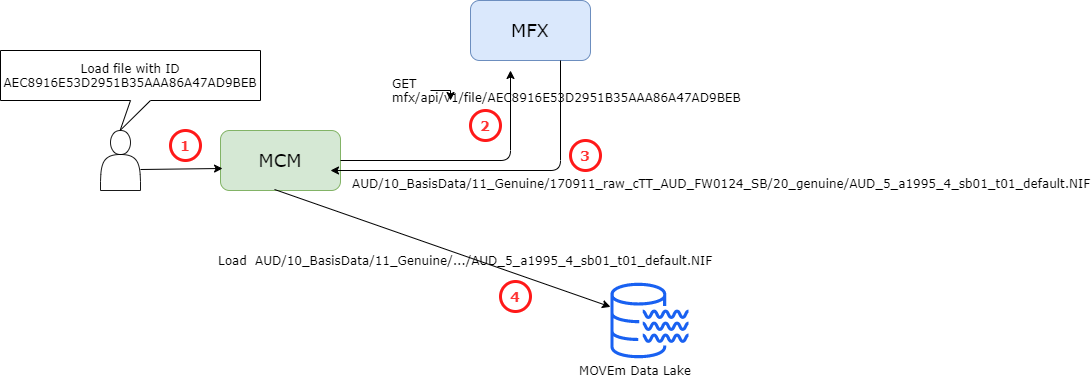
\includegraphics[width=1.0\textwidth]{images/mfx_usage.png}
  \caption{MCM uses MFX for lookup of file paths in the Data Lake}\label{fig:mfx_usage}
\end{figure}



\section{MOVEm Data Service}
MDS (MOVEm Data Service) is another REST based Flask web application, with the MDS database in the background. It allows the lookup of NIF data, namely on the levels of NIF (metadata, recording data, device data etc.), Note (all note specific data recorded by the reader, such as algorithm results or the values of the NOTEMSG2 chunk presented above), and Image (the actual note images recorded by the reader).\par Currently the MDS database stores about 322 GB of NIF data, whereas the Data Lakes stores about 6.67 TB of NIFs, which are about 1110714 (status March 2021) individual files. The MDS application also entails a NIF parsing module (movem), which on user request will crawl the entire MFX, parse each NIF file indexed in MFX and store the relevant information in the MDS database. \par The big improvement that comes with introducing MDS is that it allows lazy loading of NIF data. Depending on the use case, MDS allows fetching NIF data (metadata on the file, like the time of recording, the reader used etc.), Note data, or Image data i.e. actual images. This is a huge difference to the MCM architecture, where always the entire NIF is loaded and all images cached. In many use cases, adaptation specialists analyze algorithmic data on the level of the Note and only need to look at images in special cases. There are even NIF analyzing tools that do not support the displaying of images at all, but still unnecessarily load and cache all images, because they use and underlying MCM core for the loading of NIF data. The promise of MDS in the long run is therefore improved loading time and less use or memory, mainly due to the lazy loading of images.
 However, to achieve this goal, the architecture of the majority of the toolchain would have to be substantially changed.\par The following figure visualizes the MDS architecture, as well as the power of the MDS API\footnote{This image was created by Lukas Burger and he kindly let me borrow it for this documentation}.
\begin{figure}[ht!]
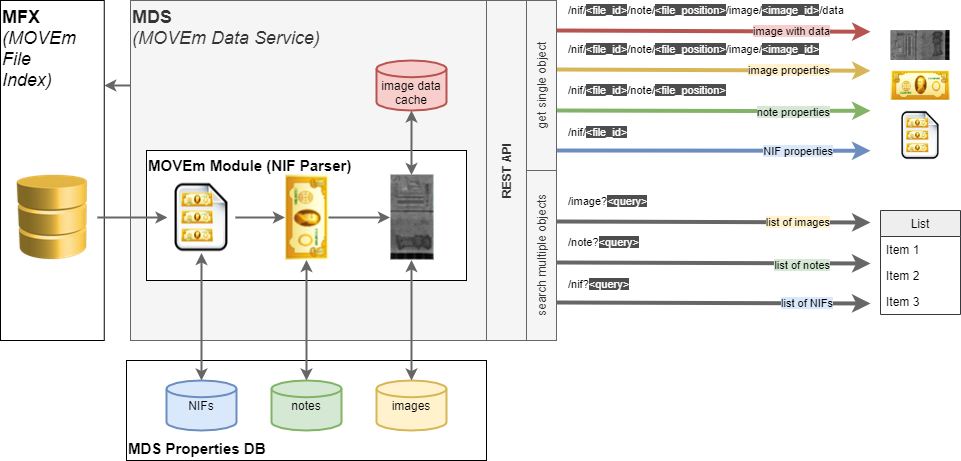
\includegraphics[width=1.0\textwidth]{images/MDS Overview.png}
  \caption{MDS architecture and API}\label{fig:mds_overview}
\end{figure}

\section{MOVEm Simulator}
The MOVEm Simulator is a user interface to the core application of the MOVEm firmware, the embedded banknote reader software. It's a desktop application written in Python and Qt and its purpose is to test currency data files (.cdf files) without the need of operating a physical banknote reader and actual physical banknotes. Input of the MOVEm simulation are existing .NIF files. The simulator then takes the raw data from these files and calculates classification, sorting and algorithm results the same way one can expect from a physical test with real banknote readers. Output of the simulation are so called Level-1 .NIF files. These are valid, minimal .NIF files which contain all the computed results, but no image data (Which of course the simulator cannot generate). 

\section{MOVE Currency Modeller}
MOVE Currency Modeller (MCM) is the adaptation specialist's main tool which they use to create and test Currency Data Files (CDF). Typically, users load raw data (NIF files) into MCM and use this data to develop. test and improve CDFs or train a particular algorithm within a CDF. MCM has an interface to the embedded software algorithmic framework and thus is able to simulate the individual algorithms used by the banknote reader. MCM is a desktop application which has been developed over years and contains a huge range of viewers and functionality. It's a very powerful tool but also a monolithic one, and as of today not very modularizable. Although MFX is already integrated into MCM as mentioned above, MDS isn't yet. The integration of MDS is in the works and comes with the promise of performance improvements, because it would allow the lazy loading of individual notesor images from the MDS API, as opposed to always having to parse and load the entire NIF, even if one just wants to look at a particular note or image therein.

\section{The Notelist Format}
\label{section:notelist}
Since the NIF file is immutable, the need to persist sets of notes requires a dedicated format. The Notelist format is an XML-based format, which is structured in a hierarchical way and consists of the following elements:
\begin{itemize}
	\item Notelist: A list of NoteContainers
	\item NoteContainer: A list of NoteItems
	\item NoteItem: Contains the annotation/label for one note
\end{itemize}
The purpose of the Notelist format was on the one hand the already mentioned possibility to group notes from different NIFs together. Another feature, is the per-note annotation (NoteItem), which allows the adaptation specialist to annotate notes differently from and independently of the reader's recognition/labeling. For example, a note might be recognized as a Class 4 (genuine) by the current CDF but the adaptation specialist knows it's actually a new type of counterfeit and thus wants to label it as a counterfeit (Class 3) when using it in the training data.\par
Notelists can be loaded in MCM and today constitute the standard means of persisting sets of notes in the context of currency adaptation.
\begin{figure}[ht!]
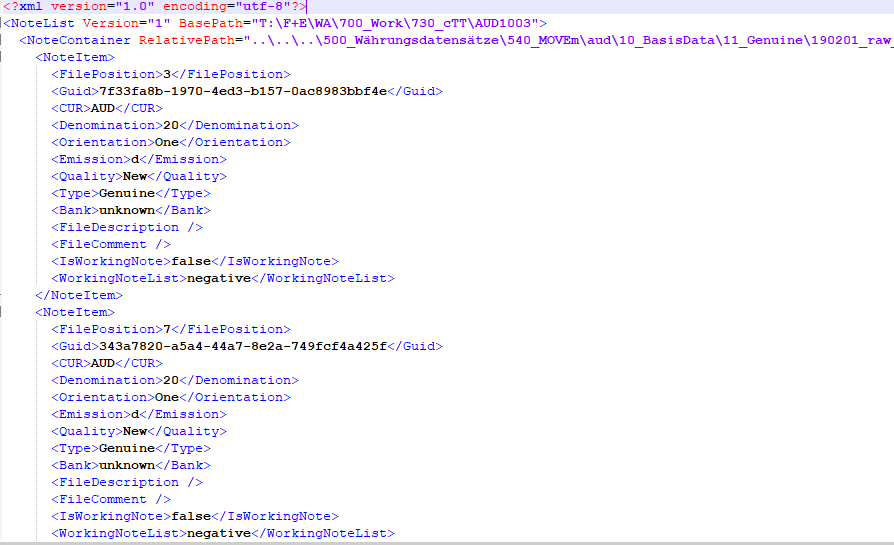
\includegraphics[width=1.0\textwidth]{images/Notelist.png}
  \caption{Extract of a Notelist file}\label{fig:notelist}
\end{figure}